\subsection{Server Utilization}
\label{subsec:server_util}

During all measurements, CPU and network utilization on the server were monitored and measured. The different results can be categorized into low latency and high latency measurements. For that reason only the server utilization for the local (low latency) and North America (high latency) measurements will be presented. The performance graph for the server CPU utilization is shown in Figure \ref{fig:cpu}.  

\begin{figure}[H]
\centering
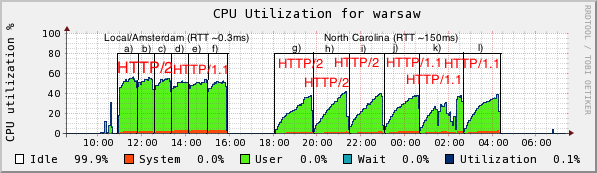
\includegraphics[scale=0.6,trim=0.0cm .0cm .0cm .0cm,clip]{images/cpu3.png}
\caption{Server CPU utilization for Local and North America measurements}
\label{fig:cpu}
\end{figure}

Table \ref{table:cpu} describes the corresponding annotations that have been made to point out which measurement belongs to which measurement parameters. That table applies also for the next performance graphs since we always show exactly the same time range in all following graphs.

\begin{table}[h]
	\centering
\begin{tabular}{ | c | c | c | }

\hline
\textbf{Index} &\textbf{Protocol} &\textbf{Web Page Size}\\ \hline \hline
a & HTTP/2 & small.html (20kB)\\ \hline
b & HTTP/2 & medium.html (600kB)\\ \hline
c & HTTP/2 & large.html (1600kB)\\ \hline
d & HTTP/1.1 & small.html (20kB) \\ \hline
e & HTTP/1.1 & medium.html (600kB) \\ \hline
f & HTTP/1.1 & large.html (1600kB)\\ \hline 
g & HTTP/2 & small.html (20kB)\\ \hline
h & HTTP/2 & medium.html (600kB)\\ \hline
i & HTTP/2 & large.html (1600kB)\\ \hline
j & HTTP/1.1 & small.html (20kB) \\ \hline
k & HTTP/1.1 & medium.html (600kB) \\ \hline
l & HTTP/1.1 & large.html (1600kB)\\  
\hline
\end{tabular}
\caption{Different Measurement parameters}
\label{table:cpu}
\end{table} 
 
The careful reader will now  notice that a medium.html web page shows up in Table \ref{table:cpu}. Indeed we created three different types of web pages. During the analysis of the data we realised that there is almost no significant difference in all measurements between the small size page and the medium size pages. For that reason we did not consider the measurements for the medium.html page and only focussed on the other two categories (large.html/small.html). However, in the performance graphs of the server the measurement for the medium size web pages are included.
\\ 
The left part of the graph shows the CPU utilization for local measurements (low latency) on the server and is annotated with the letters \textit{a} to \textit{f}. A sudden increase up to 60\% from the beginning on is remarkable until CPU utilization remains at a stable level. That correlates to the request rates graph for local measurements and nicely presents a high CPU utilization caused by the high number of requests towards the server. The measurements from \textit{a} to \textit{c} show HTTP/2 measurements and from \textit{d} to \textit{f} HTTP/1.1 measurements. A significant difference regarding CPU utilization is not noticeable. Starting from 6pm until 4am (annotated by \textit{g} to \textit{l}) measurements over a high latency link (North America) were performed. We see a constant growing of the CPU graph until the maximum number of clients of 750 for each test is reached. A nearly identical characteristic shows the bandwidth utilization graph. That correlates to the request per second graph as well and reflects a growing load caused by constantly increasing number of requests. A significant difference between HTTP/1.1 and HTTP/2 is also not noticeable for the high latency measurements. Furthermore a different load characteristic for changing sizes of web pages is not measurable for both protocol variants. 
\\
The traffic graph (Figure \ref{fig:network}) that represents the bandwidth utilization of the external interface of the server shows a similar characteristic compared to the CPU utilization graph (Figure \ref{fig:cpu}). One difference is the increased amount of traffic that can be explained by the increased amount of data for larger web pages. 

\begin{figure}[H]
\centering
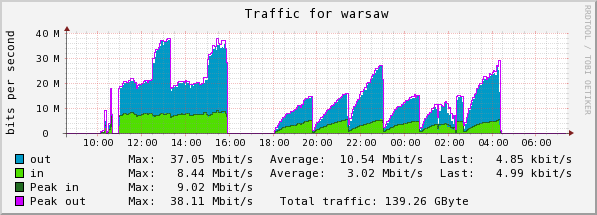
\includegraphics[scale=0.6,trim=0.0cm .0cm .0cm .0cm,clip]{images/network.png}
\caption{Server Bandwidth utilization for Local and North America measurements}
\label{fig:network}
\end{figure}

It is worth to mention that for all HTTP/1.1 measurements a lot of TCP TIME WAIT connections were discovered on the server. TCP TIME WAITS occur when the endpoint (server) blocks a current connection before it can close it due to some missing packets for that particular session. That happens because the server has many more TCP connections to manage for HTTP/1.1 compared to HTTP/2 and shows clearly the benefit of using the HTTP/2 protocol. 
The graph representing the TCP socket states on the server is shown in Figure \ref{fig:sockets}.

\begin{figure}[H]
\centering
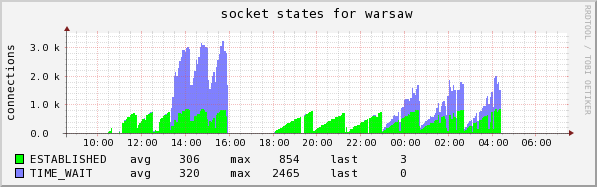
\includegraphics[scale=0.6,trim=0.0cm .0cm .0cm .0cm,clip]{images/sockets.png}
\caption{Server sockets for Local and North America measurements}
\label{fig:sockets}
\end{figure}